





\section{FFT}

Die schnelle Fourier-Transformation (FFT) ist ein Algorithmus von  James Cooley und John W. Tukey zur schnellen Berechnung der diskreten Fourier-Transformation. Mit dieser Transformation kann ein zeitdiskretes Signal $f(t)$ in ihre Frequenzanteile bzw. Frequenzspektrum zerlegt werden \cite[S.14]{hejobu 84}. Ein Frequenzspektrum beschreibt die Stärke der jeweiligen Frequenz im zu Grunde liegenden Signal. Um den FFT-Algorithmus zu verstehen, müssen kurz ein paar Grundlagen erklärt werden.


\subsection{Fourierreihe}

Die Fourierreihe ist eine Reihenentwicklung ähnlich der Taylor-Serie, die periodische Funktionen als eine unendlich Reihe von Sinus- und Cosinus-Funktionen beliebig genau approximiert kann \cite[K. 11.4]{krenor 11}. Eine periodische Funktion muss sich in Periode T wiederholen. Dem entsprechend muss gelten:
\begin{equation}
f(t) = f(t + T)
\end{equation}

Die Fourierserie besitzt folgende Form:
\begin{equation}
f(t) = \frac{a_0}{2} + \sum_{n=1}^{\infty} a_n cos \left( \frac{n2 \pi t}{T} \right) + b_n sin \left( \frac{n2 \pi t}{T} \right)
\label{eq:fourierreihe}
\end{equation}
Für die Approximation müssen die Koeffizienten $a_n$ und $b_n$ berechnet werden (für die Berechnung siehe \cite[K. 11.2]{krenor 11}). Die Koeffizienten $a_n$ und $b_n$ stehen dabei im Zusammenhang mit der Amplitude der verschiedenen Frequenzen in der Reihe \cite[K. 2.5]{scho 05}. Somit lässt sich eine periodische Funktion $f(t)$ mit der Fourierreihe in ihre Teilfrequenzen zerlegen und mit Hilfe der Koeffizienten das Frequenzspektrum anzeigen lassen (siehe Abbildung \ref{fig:fourierreihe}).
\newline
Die Entwicklung einer Funktion $f(t)$ kann auch als Zerlegung der Funktion in die durch trigonometrischen Basisfunktionen dargestellten Schwingungen verstanden werden und heißt Fourieranalyse.
\begin{figure}
\centering
 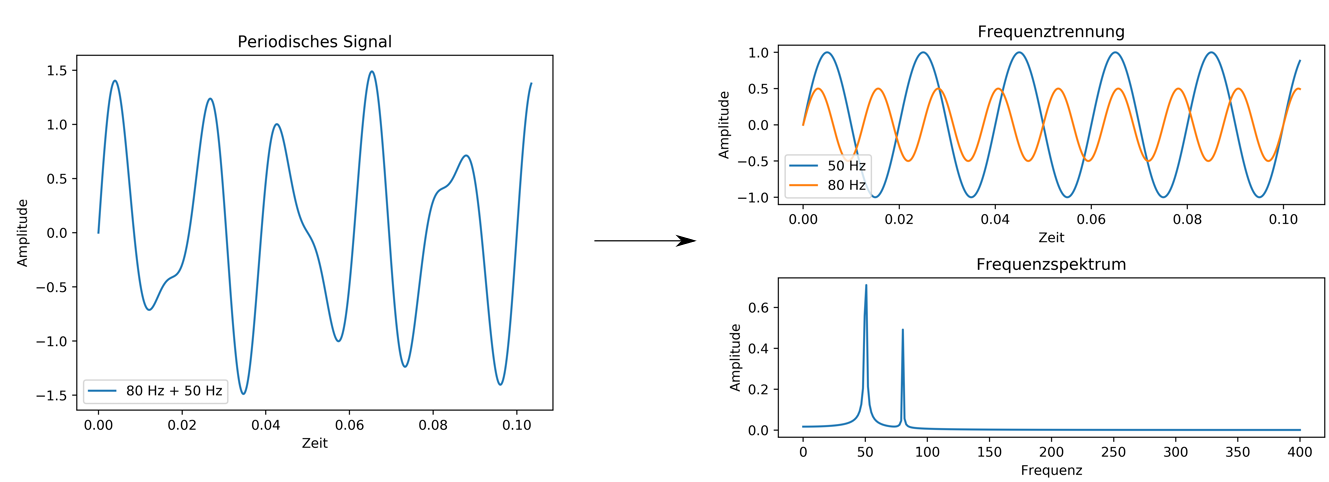
\includegraphics[width=0.8\textwidth]{Pictures/Fourierreihe.png}
\caption{Anwendung Fourierreihe}
\label{fig:fourierreihe}
\end{figure} 
\newline
Für die Fourierreihe gibt es auch eine komplexe Darstellung. Für diese muss zuerst die eulersche Formel $e^{ix} = cos(x) + i sin(x)$ umgestellt werden:
\begin{equation}
cos(x) = \frac{e^{ix} + e^{-ix}}{2}
\label{eq:euler1}
\end{equation}
\begin{equation}
sin(x) = \frac{e^{ix} - e^{-ix}}{2i}
\label{eq:euler2}
\end{equation}
Nun müssen die trigonometrischen Funktion in Formel \ref{eq:fourierreihe} mit Formel \ref{eq:euler1} und \ref{eq:euler2} ersetzt werden.
Dabei entsteht folgende Gleichung:
\begin{equation}
f(x) = \sum_{n=-\infty}^{\infty} c_{n} e^{in2\pi x / T}
\label{FS}
\end{equation}
Hierbei ist $c_n$ eine Konstante, die für die Approximation der Fourier berechnet werden muss.


\subsection{Diskrete Fouriertransformation}
Die diskrete Fouriertransformation DFT verwandelt wie die Fourierserie ein periodische Signal in ihr Frequenzspektrum um. Im Gegensatz zur Fourierreihe wird aber ein endliches zeitdiskretes Signal und kein kontinuierliches Signal verwandelt.
Deswegen ist die DFT auch besser für Algorithmen in der Informatik geeignet, da Rechner mit diskreten Werten arbeiten. Folgende Formel zeigt wie ein zeitdiskretes Signal $x_{n} = x_{1}, x_{2},...$ in ein diskretes, periodisches Frequenzspektrum $X_{k} = X_{1}, X_{2},...$ transformiert wird \cite[S.17]{and 12}:
\begin{equation}
X_{k}= \sum_{n=0}^{N-1} x_{n} e^{-i2 \pi kn /N} \text{  für } k=0,...,N-1
\label{eq:DFT}
\end{equation}

Die inverse DFT (iDFT) lautet \cite[S.20]{and 12}:
\begin{equation}
x_{k}= \frac{1}{N}\sum_{k=0}^{N-1} X_{k} e^{i2 \pi kn /N} \text{  für }  n=0,...,N-1
\label{idft}
\end{equation}
Beide Formeln lassen sich aus der komplexen Formel \ref{FS} der Fourierreihe herleiten \cite[S. 77-79]{ser 17}. Die DFT lässt sich mit Hilfe der Einheitswurzel $w_{N} = e^{-2 \pi ik /N}$ in folgende Formel vereinfachen:
\begin{equation}
X_{k}= \sum_{n=0}^{N-1} x_{n} w_{N}^{kn}
\end{equation}
Mit Hilfe der Fouriermatrix $F_{N} = (w^{kn})_{k,n=0}^{N-1}$ und der Matrixschreibweise erhalten wir folgende Formel:
\begin{equation}
X_{k} = x_{n}F_{N}
\label{eq:dft fouriermatrix}
\end{equation}
Somit ist die DFT eine Matrix-Vektor-Multiplikation zwischen einem Vektor $x_n$ und der $n*n$ Fouriermatrix.
Somit benötigt die DFT für n Elemente jeweils n Multiplikationen und für jede Multiplikation n - 1 Additionen. Es ergibt sich folgende Laufzeit: 
\begin{equation}
DFT \in \mathcal O(n^2)
\end{equation}

\subsection{Implementierung FFT}
Die schnelle Fouriertransformation FFT ist ein Algorithmus für die DFT, der durch Ausnutzen der Symmetrie der Einheitswurzel die Laufzeit des Algorithmus auf $FFT \in \mathcal O(n \log n)$ verringert.
\newline
Nach Formel \ref{eq:dft fouriermatrix} ist die DFT eine Matrix-Vektor-Multiplikation aus $x_{n}$ und der Fouriermatrix $F_{N}$:
\begin{equation}
\left( \begin{array}{cccc}
w^0 & w^0 & \cdots & w^0\\
w^0 & w^1 & \cdots & w^{N-1}\\
\vdots & \vdots & \ddots & \vdots\\
w^0 & w^{N-1} & \cdots & w^{(N-1)(N-1)}\\
\end{array}\right)
\left( \begin{array}{c}
x_0\\
x_1\\
\vdots\\
x_{N-1}
\end{array}\right)
\end{equation}
Die Idee des Verfahrens ist es die Matrix-Vektor-Multiplikation mit $N$ Elemente auf zwei Matrix-Vektor-Multiplikation mit $\frac{N}{2}$ aufzuteilen. Durch diese Aufteilung werden Rechenoperationen eingespart. Dieser Vorgang wird solange wiederholt bis nur noch ein Element in der Matrix ist. Deswegen muss $N$ eine Zweierpotenz sein. Der Algorithmus ist somit ein Teile-Herrsche-Verfahren.
Für das Aufteilen muss die Struktur der Fouriermatrix vereinfacht werden. Dies ist durch folgende Eigenschaften der $N$-ten Einheitswurzel möglich:
\begin{itemize}
\item $w^{N/2} = -1$ \text{ für $N$ gerade}
\item $w^{kN} = 1$
\end{itemize}
Zur Veranschaulichung wird der erste Schritt im Verfahren an einer $8*8$ Fouriermatrix durchgeführt:
\begin{equation*}
\left( \begin{array}{cccccccc}
w^{0} & w^{0} & w^{0} & w^{0} & w^{0} & w^{0} & w^{0} & w^{0}\\
w^{0} & w^{1} & w^{2} & w^{3} & w^{4} & w^{5} & w^{6} & w^{7}\\
w^{0} & w^{2} & w^{4} & w^{6} & w^{8} & w^{10} & w^{12} & w^{14}\\
w^{0} & w^{3} & w^{6} & w^{9} & w^{12} & w^{15} & w^{18} & w^{21}\\
w^{0} & w^{4} & w^{8} & w^{12} & w^{16} & w^{20} & w^{24} & w^{28}\\
w^{0} & w^{5} & w^{10} & w^{15} & w^{20} & w^{25} & w^{30} & w^{35}\\
w^{0} & w^{6} & w^{12} & w^{18} & w^{24} & w^{30} & w^{36} & w^{42}\\
w^{0} & w^{7} & w^{14} & w^{21} & w^{28} & w^{35} & w^{42} & w^{49}\\
\end{array} \right)
\end{equation*}
In Zeile 3, 5 und 7 kann in der rechten Hälfte die Eigenschaft $w^{kN} = 1$ ausgenutzt werden:
\begin{equation}
\left( \begin{array}{cccccccc}
w^{0} & w^{0} & w^{0} & w^{0} & w^{0} & w^{0} & w^{0} & w^{0}\\
w^{0} & w^{1} & w^{2} & w^{3} & w^{4} & w^{5} & w^{6} & w^{7}\\
w^{0} & w^{2} & w^{4} & w^{6} & w^{0} & w^{2} & w^{4} & w^{6}\\
w^{0} & w^{3} & w^{6} & w^{9} & w^{12} & w^{15} & w^{18} & w^{21}\\
w^{0} & w^{4} & w^{8} & w^{12} & w^{0} & w^{4} & w^{8} & w^{12}\\
w^{0} & w^{5} & w^{10} & w^{15} & w^{20} & w^{25} & w^{30} & w^{35}\\
w^{0} & w^{6} & w^{12} & w^{18} & w^{0} & w^{6} & w^{12} & w^{18}\\
w^{0} & w^{7} & w^{14} & w^{21} & w^{28} & w^{35} & w^{42} & w^{49}\\
\end{array} \right)
\end{equation}
In Zeile 1, 3, 5 und 7 ist die linke Hälfte gleich der rechten Hälfte.
Im nächsten Schritt wird die rechte Hälfte der Zeilen 2, 4, 6 und 8 mit der Eigenschaft $w^{kN} = 1$ vereinfacht:
\begin{equation*}
\left( \begin{array}{cccccccc}
w^{0} & w^{0} & w^{0} & w^{0} & w^{0} & w^{0} & w^{0} & w^{0}\\
w^{0} & w^{1} & w^{2} & w^{3} & w^{4} & w^{5} & w^{6} & w^{7}\\
w^{0} & w^{2} & w^{4} & w^{6} & w^{0} & w^{2} & w^{4} & w^{6}\\
w^{0} & w^{3} & w^{6} & w^{9} & w^{4} & w^{7} & w^{10} & w^{13}\\
w^{0} & w^{4} & w^{8} & w^{12} & w^{0} & w^{4} & w^{8} & w^{12}\\
w^{0} & w^{5} & w^{10} & w^{15} & w^{4} & w^{9} & w^{14} & w^{19}\\
w^{0} & w^{6} & w^{12} & w^{18} & w^{0} & w^{6} & w^{12} & w^{18}\\
w^{0} & w^{7} & w^{14} & w^{21} & w^{4} & w^{11} & w^{18} & w^{25}\\
\end{array} \right)
\end{equation*}
Im letzten Schritt wird in den Zeile 2, 4, 6 und 8 die Eigenschaft $w^{N/2} = -1$ benutzt und die Potenzen geschickt aufgeteilt:
\begin{equation*}
\left( \begin{array}{cccccccc}
w^{0} & w^{0} & w^{0} & w^{0} & w^{0} & w^{0} & w^{0} & w^{0}\\
w^{0}w^{0} & w^{1}w^{0} & w^{2}w^{0} & w^{3}w^{0} & -w^{0}w^{0} & -w^{1}w^{0} & -w^{2}w^{0} & -w^{3}w^{0}\\
w^{0} & w^{2} & w^{4} & w^{6} & w^{0} & w^{2} & w^{4} & w^{6}\\
w^{0}w^{0} & w^{1}w^{2} & w^{2}w^{4} & w^{3}w^{6} & -w^{0}w^{0} & -w^{1}w^{2} & -w^{2}w^{4} & -w^{3}w^{6}\\
w^{0} & w^{4} & w^{8} & w^{12} & w^{0} & w^{4} & w^{8} & w^{12}\\
w^{0}w^{0} & w^{1}w^{4} & w^{2}w^{8} & w^{3}w^{12} & -w^{0}w^{0} & -w^{1}w^{4} & -w^{2}w^{8} & -w^{3}w^{12}\\
w^{0} & w^{6} & w^{12} & w^{18} & w^{0} & w^{6} & w^{12} & w^{18}\\
w^{0}w^{0} & w^{1}w^{6} & w^{2}w^{12} & w^{3}w^{18} & -w^{0}w^{0} & -w^{1}w^{6} & -w^{2}w^{12} & -w^{3}w^{18}\\
\end{array} \right)
\end{equation*} 
Nun erkennt man, dass sich die Einträge in Zeile 1, 3, 5 und 7 auf der rechten Seite wiederholen. In den Zeilen 2, 4, 6, 8 wiederholt sich die rechte Seite ebenfalls. Allerdings muss hier noch der Vorfaktor mit beachtet werden.
Nun kann folgende Multiplikation 
\begin{equation*}
\left( \begin{array}{cccccccc}
w^{0} & w^{0} & w^{0} & w^{0} & w^{0} & w^{0} & w^{0} & w^{0}\\
w^{0}w^{0} & w^{1}w^{0} & w^{2}w^{0} & w^{3}w^{0} & -w^{0}w^{0} & -w^{1}w^{0} & -w^{2}w^{0} & -w^{3}w^{0}\\
w^{0} & w^{2} & w^{4} & w^{6} & w^{0} & w^{2} & w^{4} & w^{6}\\
w^{0}w^{0} & w^{1}w^{2} & w^{2}w^{4} & w^{3}w^{6} & -w^{0}w^{0} & -w^{1}w^{2} & -w^{2}w^{4} & -w^{3}w^{6}\\
w^{0} & w^{4} & w^{8} & w^{12} & w^{0} & w^{4} & w^{8} & w^{12}\\
w^{0}w^{0} & w^{1}w^{4} & w^{2}w^{8} & w^{3}w^{12} & -w^{0}w^{0} & -w^{1}w^{4} & -w^{2}w^{8} & -w^{3}w^{12}\\
w^{0} & w^{6} & w^{12} & w^{18} & w^{0} & w^{6} & w^{12} & w^{18}\\
w^{0}w^{0} & w^{1}w^{6} & w^{2}w^{12} & w^{3}w^{18} & -w^{0}w^{0} & -w^{1}w^{6} & -w^{2}w^{12} & -w^{3}w^{18}\\
\end{array} \right)
\left( \begin{array}{cccccccc}
x_1\\
x_2\\
x_3\\
x_4\\
x_5\\
x_6\\
x_7\\
x_8\\
\end{array} \right)
=
\left( \begin{array}{cccccccc}
b_1\\
b_2\\
b_3\\
b_4\\
b_5\\
b_6\\
b_7\\
b_8\\
\end{array} \right)
\end{equation*}
folgendermaßen aufgeteilt werden:
\begin{equation*}
\left( \begin{array}{cccc}
w^{0} & w^{0} & w^{0} & w^{0}\\
w^{0} & w^{2} & w^{4} & w^{6}\\
w^{0} & w^{4} & w^{8} & w^{12}\\
w^{0} & w^{6} & w^{12} & w^{18}\\
\end{array} \right)
\left( \begin{array}{cccc}
x_1 + x_5\\
x_2 + x_6\\
x_3 + x_7\\
x_4 + x_8\\
\end{array} \right)
=
\left( \begin{array}{cccc}
b_1\\
b_3\\
b_5\\
b_7\\
\end{array} \right)
\end{equation*} 
\begin{equation*}
\left( \begin{array}{cccc}
w^{0} & w^{0} & w^{0} & w^{0}\\
w^{0} & w^{2} & w^{4} & w^{6}\\
w^{0} & w^{4} & w^{8} & w^{12}\\
w^{0} & w^{6} & w^{12} & w^{18}\\
\end{array} \right)
\left( \begin{array}{cccc}
w^{0}(x_1 + x_5)\\
w^{1}(x_2 + x_6)\\
w^{2}(x_3 + x_7)\\
w^{3}(x_4 + x_8)\\
\end{array} \right)
=
\left( \begin{array}{cccc}
b_2\\
b_4\\
b_6\\
b_8\\
\end{array} \right)
\end{equation*} 
Beide Matrizen besitzen wieder die Form einer Fouriermatrix und können wieder aufgeteilt werden, bis nur noch ein Element in der Matrix ist.
Im Schmetterlingsdiagram in Abb. \ref{fig:schmetterlingsdiagram} wird der Algorithmus noch einmal zusammengefasst.
\begin{figure}
\centering
 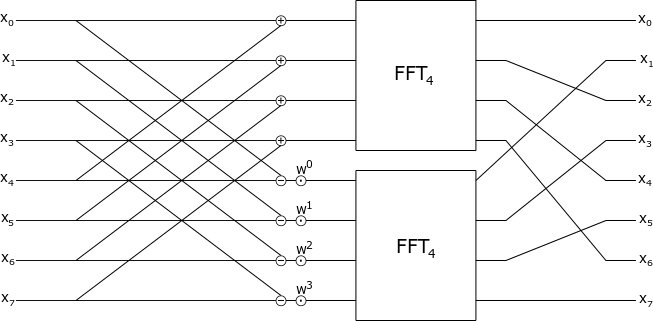
\includegraphics[width=0.8\textwidth]{Pictures/FFT.png}
\caption{Schmetterlingsdiagramm}
\label{fig:schmetterlingsdiagram}
\end{figure} 
Hier zu erkennen, dass am Ende die Elemente noch richtig sortiert werden müssen. 

\section{3D FFT}
Die 3 dimensionale FFT (3D FFT) wird in vielen verschiedenen Anwendungsbereichen benötigt.
In der Molekulardynamik zum Beispiel werden Simulationen von den physikalischen Bewegungen der Atome und Moleküle durchgeführt. Mit Hilfe des 3D FFT wird die Komplexität dieser Simulation verringert \cite[S.1]{shahe 14}.
\newline
Die 3D DFT ist definiert als \cite[S.4]{sig 07}:
\begin{equation}
F(k_x,k_y, k_z)= \sum_{j_x=0}^{N-1} \sum_{j_y=0}^{N-1} \sum_{j_x=0}^{N-1} 
f(j_x,j_y, j_z) e^{-2 \pi i \left( \frac{k_x j_x}{N_x} + \frac{k_y j_y}{N_y} + \frac{k_z j_z}{N_z} \right)}
\label{3dfft}
\end{equation}
Hierbei ist $f(x, y, z)$ ein 3 dimensionales Input-Array mit der Größe $N_x * N_y * N_z$ und $F(k_x,k_y, k_z)$ ein 3 dimensionales Output-Array.
Formel \ref{3dfft} kann in die folgende Form umgeschrieben werden:
\begin{equation}
F(k_x,k_y, k_z)= \sum_{j_x=0}^{N-1} \left( \sum_{j_y=0}^{N-1} \left( \sum_{j_x=0}^{N-1} 
f(j_x,j_y, j_z) e^{-2 \pi i \left( \frac{k_z j_z}{N_z} \right)} \right) e^{-2 \pi i \left( \frac{k_y j_y}{N_y} \right)} \right) e^{-2 \pi i \left( \frac{k_x j_x}{N_x} \right)}
\end{equation}
Dies zeigt das der drei dimensionale Fall als drei seperate ein dimesionale DFT berechent werden kann. Zuerst wird die DFT über die Z-Dimension berechnet. Dies führt zu folgenden Resultat:
\begin{equation}
F(j_x,j_y, k_z)=\sum_{j_x=0}^{N-1} 
f(j_x,j_y, j_z) e^{-2 \pi i \left( \frac{k_z j_z}{N_z} \right)}
\label{eq3dz}
\end{equation}
Die gleiche Methode wird auf die Y-Dimenstion angewendet:
\begin{equation}
F(j_x,k_y, k_z)=\sum_{j_x=0}^{N-1} 
f(j_x,j_y, j_z) e^{-2 \pi i \left( \frac{k_y j_y}{N_y} \right)}
\label{eq3dy}
\end{equation}
Zum Schluss wird noch die X-Dimension berechnet:
\begin{equation}
F(k_x,k_y, k_z)=\sum_{j_x=0}^{N-1} 
f(j_x,j_y, j_z) e^{-2 \pi i \left( \frac{k_x j_x}{N_x} \right)}
\label{eq3dx}
\end{equation}
Die Reihenfolge der Dimensionen ist nicht relevant für die 3D DFT \cite[S.3-4]{sig 07}.
Die einzelnen 1D DFT können nun mit dem 1D FFT berechnet werden.

\section{FFT-ECP Implementierung}
Das FFT-ECP Projekt soll eine nachhaltige 3D FFT Bibliothek für verteilte-heterogene parallele Systeme zur Verfügung stellen. Dies wird von dem Exascale Computing Project (ECP), welches vom US Department of Energy finanziert wird, entwickelt \cite[S. 1]{sha 19}. 
\newline
FFT-ECP basiert auf FFTMPI, eine CPU-FFT Bibliothek, die von dem Sandia National Laboratory entwickelt wurde. Diese Bibliothek kann 3D- oder 2D-FFTs parallel auf verteilten Prozessoren durchführen. Momentan werden GPUs nicht unterstützt. Ein wichtiges Feature von FFTMPI ist die Flexilibität des Input- und Output-Layers \cite[S.2]{sha 19}. 
\newline
Der Algorithmus für die 3D FFT schaut wie folgt aus:
\newline
Der 3D FFT Algorithmus basiert auf der sogenannten Pencil decomposition \cite[S.1-2]{aya 19}.
Die Input-Daten sind ein 3D Tensor mit folgende Dimensionen $N_{x} * N_{y} * N_{z}$ (siehe Abb. \ref{fig:pencildecomposition} a). Die Daten werden auf einem Gitter von $P$ Prozessen verteilt, $P=P_0 * P_1 * P_1$. Wie im vorherigen Kapitel beschrieben, kann die 3D FFT in drei seperate 1D FFT aufgeteilt werden. Dazu müssen die Daten in sogenannte Pencils umgeformt werden. 
\newline
Im ersten Schritt werden die Pencils entlang der X-Achse geformt (siehe Abb. \ref{fig:pencildecomposition} b). Die Pencils werden auf die $P$ Prozesse verteilt und mit 1D FFTs berechnet. Es müssen $N_y * N_{z}$ FFTs berechnet werden. Danach müssen die Daten wieder umgeformt werden. 
\newline
Im zweiten Schritt werden Pencils entlang der Y-Achse gebildet (siehe Abb. \ref{fig:pencildecomposition} c). Die Pencils werden wieder auf die $P$ Prozesse verteilt und es werden $N_x * N_z$ 1D FFTs berechnet. 
\newline
Im dritten Schritt werden die Daten in Pencils entlang der Z-Achse umgeformt, verteilt und $N_x * N_y$ 1D FFTs berechnet (siehe Abb. \ref{fig:pencildecomposition} d). Zum Schluss werden die Daten noch einmal umgeformt, um sie in die Originalform zu bringen. 
\newline
Der Algorithmus benötigt somit 4 Phasen zum Umformen der Daten und 3 Phasen zum Berechnen der 1D FFTs. Das Umformen der Daten basiert auf dem Message Passing Interface(MPI). Die 1D FFTs werden von externen Bibliotheken berechnet.

\begin{figure}
\centering
 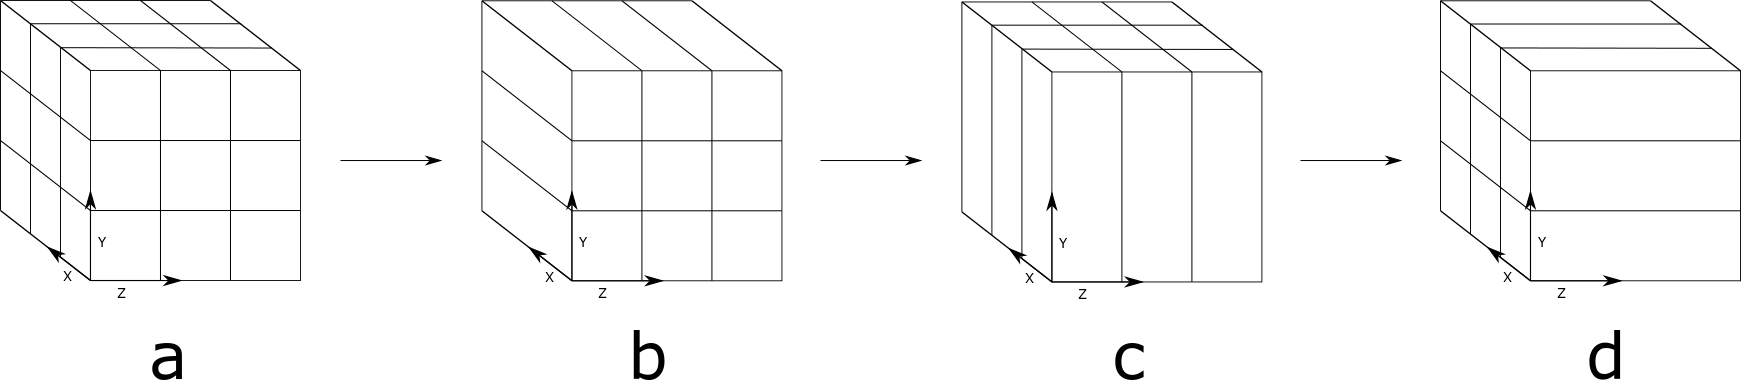
\includegraphics[width=0.8\textwidth]{Pictures/PencilsDecomposition.png}
\caption{Pencil Decomposition}
\label{fig:pencildecomposition}
\end{figure} 





